\documentclass[a4paper,12pt,twoside]{memoir}

% Castellano
\usepackage[spanish,es-tabla]{babel}
\selectlanguage{spanish}
\usepackage[utf8]{inputenc}
\usepackage[T1]{fontenc}
\usepackage{lmodern} % scalable font
\usepackage{microtype}
\usepackage{placeins}

\RequirePackage{booktabs}
\RequirePackage[table]{xcolor}
\RequirePackage{xtab}
\RequirePackage{multirow}

% Links
\usepackage[colorlinks]{hyperref}
\hypersetup{
	allcolors = {red}
}

% Ecuaciones
\usepackage{amsmath}

% Rutas de fichero / paquete
\newcommand{\ruta}[1]{{\sffamily #1}}

% Párrafos
\nonzeroparskip


% Imagenes
\usepackage{graphicx}
\newcommand{\imagen}[2]{
	\begin{figure}[!h]
		\centering
		\includegraphics[width=0.9\textwidth]{#1}
		\caption{#2}\label{fig:#1}
	\end{figure}
	\FloatBarrier
}

\newcommand{\imagenflotante}[2]{
	\begin{figure}%[!h]
		\centering
		\includegraphics[width=0.9\textwidth]{#1}
		\caption{#2}\label{fig:#1}
	\end{figure}
}



% El comando \figura nos permite insertar figuras comodamente, y utilizando
% siempre el mismo formato. Los parametros son:
% 1 -> Porcentaje del ancho de página que ocupará la figura (de 0 a 1)
% 2 --> Fichero de la imagen
% 3 --> Texto a pie de imagen
% 4 --> Etiqueta (label) para referencias
% 5 --> Opciones que queramos pasarle al \includegraphics
% 6 --> Opciones de posicionamiento a pasarle a \begin{figure}
\newcommand{\figuraConPosicion}[6]{%
  \setlength{\anchoFloat}{#1\textwidth}%
  \addtolength{\anchoFloat}{-4\fboxsep}%
  \setlength{\anchoFigura}{\anchoFloat}%
  \begin{figure}[#6]
    \begin{center}%
      \Ovalbox{%
        \begin{minipage}{\anchoFloat}%
          \begin{center}%
            \includegraphics[width=\anchoFigura,#5]{#2}%
            \caption{#3}%
            \label{#4}%
          \end{center}%
        \end{minipage}
      }%
    \end{center}%
  \end{figure}%
}

%
% Comando para incluir imágenes en formato apaisado (sin marco).
\newcommand{\figuraApaisadaSinMarco}[5]{%
  \begin{figure}%
    \begin{center}%
    \includegraphics[angle=90,height=#1\textheight,#5]{#2}%
    \caption{#3}%
    \label{#4}%
    \end{center}%
  \end{figure}%
}
% Para las tablas
\newcommand{\otoprule}{\midrule [\heavyrulewidth]}
%
% Nuevo comando para tablas pequeñas (menos de una página).
\newcommand{\tablaSmall}[5]{%
 \begin{table}
  \begin{center}
   \rowcolors {2}{gray!35}{}
   \begin{tabular}{#2}
    \toprule
    #4
    \otoprule
    #5
    \bottomrule
   \end{tabular}
   \caption{#1}
   \label{tabla:#3}
  \end{center}
 \end{table}
}

%
%Para el float H de tablaSmallSinColores
\usepackage{float}

%
% Nuevo comando para tablas pequeñas (menos de una página).
\newcommand{\tablaSmallSinColores}[5]{%
 \begin{table}[H]
  \begin{center}
   \begin{tabular}{#2}
    \toprule
    #4
    \otoprule
    #5
    \bottomrule
   \end{tabular}
   \caption{#1}
   \label{tabla:#3}
  \end{center}
 \end{table}
}

\newcommand{\tablaApaisadaSmall}[5]{%
\begin{landscape}
  \begin{table}
   \begin{center}
    \rowcolors {2}{gray!35}{}
    \begin{tabular}{#2}
     \toprule
     #4
     \otoprule
     #5
     \bottomrule
    \end{tabular}
    \caption{#1}
    \label{tabla:#3}
   \end{center}
  \end{table}
\end{landscape}
}

%
% Nuevo comando para tablas grandes con cabecera y filas alternas coloreadas en gris.
\newcommand{\tabla}[6]{%
  \begin{center}
    \tablefirsthead{
      \toprule
      #5
      \otoprule
    }
    \tablehead{
      \multicolumn{#3}{l}{\small\sl continúa desde la página anterior}\\
      \toprule
      #5
      \otoprule
    }
    \tabletail{
      \hline
      \multicolumn{#3}{r}{\small\sl continúa en la página siguiente}\\
    }
    \tablelasttail{
      \hline
    }
    \bottomcaption{#1}
    \rowcolors {2}{gray!35}{}
    \begin{xtabular}{#2}
      #6
      \bottomrule
    \end{xtabular}
    \label{tabla:#4}
  \end{center}
}

%
% Nuevo comando para tablas grandes con cabecera.
\newcommand{\tablaSinColores}[6]{%
  \begin{center}
    \tablefirsthead{
      \toprule
      #5
      \otoprule
    }
    \tablehead{
      \multicolumn{#3}{l}{\small\sl continúa desde la página anterior}\\
      \toprule
      #5
      \otoprule
    }
    \tabletail{
      \hline
      \multicolumn{#3}{r}{\small\sl continúa en la página siguiente}\\
    }
    \tablelasttail{
      \hline
    }
    \bottomcaption{#1}
    \begin{xtabular}{#2}
      #6
      \bottomrule
    \end{xtabular}
    \label{tabla:#4}
  \end{center}
}

%
% Nuevo comando para tablas grandes sin cabecera.
\newcommand{\tablaSinCabecera}[5]{%
  \begin{center}
    \tablefirsthead{
      \toprule
    }
    \tablehead{
      \multicolumn{#3}{l}{\small\sl continúa desde la página anterior}\\
      \hline
    }
    \tabletail{
      \hline
      \multicolumn{#3}{r}{\small\sl continúa en la página siguiente}\\
    }
    \tablelasttail{
      \hline
    }
    \bottomcaption{#1}
  \begin{xtabular}{#2}
    #5
   \bottomrule
  \end{xtabular}
  \label{tabla:#4}
  \end{center}
}



\definecolor{cgoLight}{HTML}{EEEEEE}
\definecolor{cgoExtralight}{HTML}{FFFFFF}

%
% Nuevo comando para tablas grandes sin cabecera.
\newcommand{\tablaSinCabeceraConBandas}[5]{%
  \begin{center}
    \tablefirsthead{
      \toprule
    }
    \tablehead{
      \multicolumn{#3}{l}{\small\sl continúa desde la página anterior}\\
      \hline
    }
    \tabletail{
      \hline
      \multicolumn{#3}{r}{\small\sl continúa en la página siguiente}\\
    }
    \tablelasttail{
      \hline
    }
    \bottomcaption{#1}
    \rowcolors[]{1}{cgoExtralight}{cgoLight}

  \begin{xtabular}{#2}
    #5
   \bottomrule
  \end{xtabular}
  \label{tabla:#4}
  \end{center}
}




\graphicspath{ {./img/} }

% Capítulos
\chapterstyle{bianchi}
\newcommand{\capitulo}[2]{
	\setcounter{chapter}{#1}
	\setcounter{section}{0}
	\chapter*{#2}
	\addcontentsline{toc}{chapter}{#2}
	\markboth{#2}{#2}
}

% Apéndices
\renewcommand{\appendixname}{Apéndice}
\renewcommand*\cftappendixname{\appendixname}

\newcommand{\apendice}[1]{
	%\renewcommand{\thechapter}{A}
	\chapter{#1}
}

\renewcommand*\cftappendixname{\appendixname\ }

% Formato de portada
\makeatletter
\usepackage{xcolor}
\newcommand{\tutor}[1]{\def\@tutor{#1}}
\newcommand{\course}[1]{\def\@course{#1}}
\definecolor{cpardoBox}{HTML}{E6E6FF}
\def\maketitle{
  \null
  \thispagestyle{empty}
  % Cabecera ----------------
\noindent
\includegraphics[width=\textwidth]{cabecera}\vspace{1cm}%
  \vfill
  % Título proyecto y escudo informática ----------------
  \colorbox{cpardoBox}{%
    \begin{minipage}{.8\textwidth}
      \vspace{.5cm}\Large
      \begin{center}
      \textbf{TFG del Grado en Ingeniería Informática}\vspace{.6cm}\\
      \textbf{\LARGE\@title{}}
      \end{center}
      \vspace{.2cm}
    \end{minipage}

  }%
  \hfill\begin{minipage}{.20\textwidth}
    
\includegraphics[width=\textwidth]{escudoInfor}
  \end{minipage}
  \vfill
  % Datos de alumno, curso y tutores ------------------
  \begin{center}%
  {%
    \noindent\LARGE
    Presentado por \@author{}\\ 
    en Universidad de Burgos --- \@date{}\\
    Tutor: \@tutor{}\\
  }%
  \end{center}%
  \null
  \cleardoublepage
  }
\makeatother


% Datos de portada
\title{Jellyfish Forecast \\Documentación Técnica}
\author{Pablo Santidrian Tudanca}
\tutor{José Francisco Díez Pastor y Álvar Arnaiz González}
\date{\today}

\begin{document}

\maketitle



\cleardoublepage



%%%%%%%%%%%%%%%%%%%%%%%%%%%%%%%%%%%%%%%%%%%%%%%%%%%%%%%%%%%%%%%%%%%%%%%%%%%%%%%%%%%%%%%%



\frontmatter


\clearpage

% Indices
\tableofcontents

\clearpage

\listoffigures

\clearpage

\listoftables

\clearpage

\mainmatter

\appendix

\apendice{Plan de Proyecto Software}

\section{Introducción}

En el siguiente apéndice se incluye la evolución temporal que ha tenido del proyecto durante la realización del mismo, además de aspectos relevantes del diseño y económicos que afectarán a su viabilidad.	

\section{Planificación temporal}

En este apartado se procederá a explicar con detalle cuál ha sido el resultado de la planificación del proyecto. Está planificación se ha realizado utilizando una metodología ágil basada en \emph{sprints} de una duración de una o dos semanas en función de las necesidades y el tiempo disponible debido a otras cargas de trabajo diferentes a este proyecto.

En estos \emph{sprints} se van marcando ciertos objetivos que serán revisados junto a los tutores en las reuniones al final de los mismos. Los objetivos del siguiente \emph{sprint} serán marcados durante dichas reuniones.

Para el control de tiempos se ha utilizado la herramienta ZenHub siendo la valoración de los \emph{Story Points} la siguiente:

\tablaSmall{Equivalencias \emph{Story Points} y tiempo estimado}{c c }{StoryPoints/tiempo}
{ \multicolumn{1}{l}{Story Points} & Estimación temporal \\}{ 
	1            & 1 hora              \\ 
	2            & 1,5 horas           \\ 
	3            & 2 horas             \\ 
	4            & 2,5 horas           \\ 
	5            & 3 horas             \\ 
	6            & 3,5 horas           \\ 
	7            & 4 horas             \\ 
	8            & 6 horas             \\ 
	9            & 9 horas             \\ 
}

%Aclarar que los gráficos \emph{Burn Down} de los primeros \emph{sprints} no están todo lo bien que deberían por la poca experiencia con la herramienta.

\subsection{Sprint 1 (29/01/2020 - 05/02/2020)}\label{Sprint-1}
En esta primera reunión se marcó el comienzo del proyecto. Ya se había hablado anteriormente con uno de los tutores (Jose Francisco) del interés sobre el proyecto propuesto del que también formaba parte de los tutores Álvar Arnaiz.

Al ser la primera reunión se habló de las herramientas que se iban a utilizar así como acordar los primeros objetivos de este \emph{sprint}:

\begin{itemize}
\item Crear el repositorio.
\item Añadir la plantilla de \LaTeX{} a la documentación.
\item Crear cuenta en la plataforma \emph{Copernicus}.
\item Investigar el funcionamiento básico de las librerías a utilizar.
\item Leer una serie de papers que me proporcionaron sobre las medusas.
\end{itemize}

Las \emph{issues} para este \emph{Sprint} se pueden ver \href{https://github.com/psnti/TFG-Pablo-Santidrian-Tudanca/milestone/1}{aquí}.

Se estimó unas 10 horas de trabajo de las que finalmente se invirtieron 8 horas quedando sin terminar una \emph{issue}.

\imagen{Sprint1_BurnDown.png}{\textit{Burndown chart} del Sprint 1}

\subsection{Sprint 2 (13/02/2020 - 28/02/2020)}\label{Sprint-2}

En la segunda reunión se comentó la existencia de una API para la descarga de los datos meteorológicos como alternativa a la descarga de una gran cantidad de datos a través del FTP.

Por otro lado, se me proporcionó apuntes de la asignatura de minería de datos para su lectura y aprendizaje.

Por último, los tutores me recomendaron iniciar la documentación del plan de proyecto de los \emph{Sprints} que se fuesen sucediendo para no acumular trabajo y se pudiera olvidar detalles del mismos.

Los objetivos fueron los siguientes:

\begin{itemize}
\item Realizar script para la descarga de los datos.
\item Comenzar a documentar el plan del proyecto.
\item Lectura de apuntes y papers.
\end{itemize}

Las \emph{issues} para este \emph{Sprint} se pueden ver \href{https://github.com/psnti/TFG-Pablo-Santidrian-Tudanca/milestone/2}{aquí}.

Se estimaron unas 8 horas de trabajo de las que finalmente se invirtieron 9 horas.

\imagen{Sprint2_BurnDown.png}{\textit{Burndown chart} del Sprint 2}

\subsection{Sprint 3 (28/02/2020 - 17/03/2020)}\label{Sprint-3}

En esta tercera reunión hablamos sobre la descarga de los datos, de las dos opciones posibles nos quedamos con la descarga por FTP por ser más fiable. Además este \emph{Sprint} se centrará en su mayor parte en documentación como las herramientas a utilizar o cuestiones teóricas sobre las medusas aparte de comenzar a desarrollar la base de la aplicación web.

Se marcaron los siguientes objetivos:
\begin{itemize}
\item Comienzo desarrollo web.
\item Elaboración de parte de la documentación teórica.
\item Descarga de los datos en un equipo de cómputo habilitado en la Universidad.
\end{itemize}

Las \emph{issues} para este \emph{Sprint} se pueden ver \href{https://github.com/psnti/TFG-Pablo-Santidrian-Tudanca/milestone/3}{aquí}.

Se estimó unas 19 horas y finalmente se realizaron 24. La causa del desvió de horas principalmente fueron: el comienzo del desarrollo web por el desconocimiento previo y el comentar el código creado para la descarga de los datos necesarios pues se corrigieron errores y se mejoró la salida por pantalla con una barra de descarga más visual.


\imagen{Sprint3_BurnDown.png}{\textit{Burndown chart} del Sprint 3}

\subsection{Sprint 4 (17/03/2020 - 30/03/2020)}\label{Sprint-4}

La cuarta reunión se hizo mediante \emph{Skype} con José Francisco debido a la cuarentena por el coronavirus. Se habló sobre la necesidad de utilizar la VPN de la universidad por este mismo motivo para poder tener acceso a la maquina remota. 

Por otra parte, se mostró el avance de la web acordando que el siguiente paso debería ser la introducción de los mapas para lo que se comentaron varias bibliotecas de las que se podía hacer uso.

Los objetivos que se marcaron fueron:
\begin{itemize}
	\item Continuación desarrollo web.
	\item Introducción de mapas en la aplicación web.
	\item Conexión a la VPN de la universidad para conseguir dejar los datos descargándose aunque la sesión esté cerrada.
	\item Continuación de la documentación.
\end{itemize}

Las \emph{issues} para este \emph{Sprint} se pueden ver \href{https://github.com/psnti/TFG-Pablo-Santidrian-Tudanca/milestone/4}{aquí}.

\imagen{Sprint4_BurnDown.png}{\textit{Burndown chart} del Sprint 4}

Se estimaron 15 hora y media y finalmente se realizaron 16.

\subsection{Sprint 5 (30/03/2020 - 14/4/2020)}\label{Sprint-5}

Esta reunión se realizó también de manera remota por \emph{Skype} con ambos tutores. Se mostró la implementación de los mapas en la aplicación web así como varias mejoras en la interfaz de la misma. También avances realizados en la memoria y ciertas mejoras propuestas por los tutores.

Sobre la web, a pesar de haber empezado su desarrollo, se recomendó el realizar unos bocetos de la misma para definir la estructura a seguir.

Por otro lado, una vez descargados los datos oceánicos el siguiente paso será generar una estructura de datos para poder entrenar al modelo.

Por último, se acordó que el siguiente paso en la realización de la memoria debía ser la finalización de los objetivos del proyecto y definir los requisitos.

Los objetivos que se marcaron fueron los siguientes:
\begin{itemize}
	\item Generar estructura de datos.
	\item Definir objetivos del proyecto.
	\item Definir requisitos.
	\item Definir aspectos relevantes.
	\item Realizar bocetos aplicación web.
\end{itemize}

Las \emph{issues} para este \emph{Sprint} se pueden ver \href{https://github.com/psnti/TFG-Pablo-Santidrian-Tudanca/milestone/5}{aquí}.

\imagen{Sprint5_BurnDown.png}{\textit{Burndown chart} del Sprint 5}

Se estimaron 12,5 horas y finalmente se realizaron 18,5.

\subsection{Sprint 6 (15/4/2020 - 24/4/2020)}\label{Sprint-6}

%Comentarios reunión.
En esta reunión se mostró los avances realizados en la generación de la estructura de datos que posteriormente se utilizará en la creación del modelo de predicción. Se comentaron diferentes problemas encontrados como la existencia de valores nulos es los datos de origen así como la mejor forma de localizar los cuadrantes contiguos a las playas.\\
También cambios realizados en la memoria y anexos.

Para este sprint se marcaron como objetivo:
\begin{itemize}
	\item Añadir mas cuadrantes a la estructura de datos mencionada así como asegurar la selección de los cuadrantes contiguos a las playa.
	\item Redacción de casos de uso.
	\item Investigar el despliegue de la página web.
	\item Añadir diferentes partes  documentación.
\end{itemize} 

Las \emph{issues} para este \emph{Sprint} se pueden ver \href{https://github.com/psnti/TFG-Pablo-Santidrian-Tudanca/milestone/6}{aquí}.

%Gráfico
\imagen{Sprint6_BurnDown.png}{\textit{Burndown chart} del Sprint 6}

%Estimación horas
En un principio se estimaron 16 horas y media y finalmente se realizaron 21 horas.

\subsection{Sprint 7 (25/4/2020 - 8/5/2020)}\label{Sprint-7}

%Comentarios reunión.
La temática de la reunión de este sprint fue similar a la anterior. Se habían solucionado los problemas con los valores nulos y añadido más cuadrantes a la estructura de datos, esto dio lugar a algunos problemas por la orientación de las playas. Por este motivo se revisarán las playas para ver si es posible recudir el numero de las mismas y así hacer un predicción más precisa.\\
En relación a esto, se empezará con la realización del modelo predictivo aprendiendo la utilización de la biblioteca \emph{scikitLearn}.
Por ultimo, se mostró el auto despliegue de la aplicación web con \emph{heroku} desde un repositorio a parte del original.

Para este sprint se marcaron como objetivo:
\begin{itemize}
	\item Mejoras en la interfaz de la aplicación web.
	\item Revisar los datos obtenidos de las playas para reducir el dataSet inicial si fuese necesario.
	\item Aprender la utilización de scikitLearn.
	\item Corrección y ampliación de anexos y memoria.
\end{itemize} 

Las \emph{issues} para este \emph{Sprint} se pueden ver \href{https://github.com/psnti/TFG-Pablo-Santidrian-Tudanca/milestone/7}{aquí}.

%Gráfico
\imagen{Sprint7_BurnDown.png}{\textit{Burndown chart} del Sprint 7}

%Estimación horas
En un principio se estimaron 20 horas y finalmente se realizaron 27.

\subsection{Sprint 8 (12/5/2020 - 2/6/2020)}\label{Sprint-8}

Esta reunión se basó principalmente en la realización del modelo. Se comentó algunas correcciones en la estructura de los datos (valores nulos, desfase temporal en la organización de los avistamientos).

Por otra parte, hablamos de diferentes algoritmos de minería de datos que podría utilizar para realizar pruebas y con los que se obtienen mejores resultados así como otras transformaciones que realizar a la estructura de datos para lograr mejores resultado como la normalización de los datos o dar más importancia a unas clases que otras.

Para este sprint se marcaron como objetivo:
\begin{itemize}
	\item Arreglos en la estructura de datos.
	\item Investigar los diferentes algoritmos.
	\item Probar algoritmos de minería de datos.
	\item Documentar las pruebas y teoría de minería de datos.
\end{itemize} 

Las \emph{issues} para este \emph{Sprint} se pueden ver \href{https://github.com/psnti/TFG-Pablo-Santidrian-Tudanca/milestone/8}{aquí}.

%Gráfico
\imagen{Sprint8_BurnDown.png}{\textit{Burndown chart} del Sprint 7}

%Estimación horas
En un principio se estimaron 12 horas y finalmente se realizaron 20.

\subsection{Sprint 9 (3/6/2020 - 10/6/2020)}\label{Sprint-9}
La reunión estuvo basada en los algoritmos de predicción a utilizar. Se mostraron los diferentes algoritmos probados con algunos resultados y se propuso por parte de los tutores la prueba de alguno más.

Aparte de esto, hablamos sobre la necesidad de tratar los datos como series temporales debido a la naturaleza de los mismos. También se obtuvo un nuevo excel con un mayor numero de lecturas de las que se tenia hasta el momento.


Para este sprint se marcaron como objetivo:
\begin{itemize}
	\item Seguir realizando pruebas con diferentes algoritmos de minería.
	\item Investigar sobre las series temporales.
	\item Tratar nuevo Excel.
\end{itemize} 

Las \emph{issues} para este \emph{Sprint} se pueden ver \href{https://github.com/psnti/TFG-Pablo-Santidrian-Tudanca/milestone/9}{aquí}.

Gráfico
\imagen{Sprint9_BurnDown.png}{\textit{Burndown chart} del Sprint 7}

%Estimación horas
En un principio se estimaron XX horas y finalmente se realizaron XX.

\subsection{Sprint 10 (10/6/2020 - 17/6/2020)}\label{Sprint-10}

La temática de la reunión fue la misma que las anteriores. Las pruebas realizadas aplicando las series temporales a los modelos no aportaron buenos resultados por lo que se decidió realizar estas con validación cruzada y viendo que algoritmo arroja mejores resultados, utilizarlo finalmente con las series temporales.

En cuanto a la página web, se mostró la introducción de algunas funcionalidades viendo que existían bugs que subsanar.

Para este sprint se marcaron como principales objetivo:
\begin{itemize}
	\item Pruebas de algoritmos con validación cruzada.
	\item Arreglar fallos e introducir gráfico en la página web.
\end{itemize} 

Las \emph{issues} para este \emph{Sprint} se pueden ver \href{https://github.com/psnti/TFG-Pablo-Santidrian-Tudanca/milestone/10}{aquí}.

%Gráfico
%\imagen{Sprint9_BurnDown.png}{\textit{Burndown chart} del Sprint 7}

%Estimación horas
En un principio se estimaron XX horas y finalmente se realizaron XX.

\section{Estudio de viabilidad}

\subsection{Viabilidad económica}

\subsection{Viabilidad legal}



\apendice{Especificación de Requisitos}

\section{Introducción}
En este apéndice se recogerán los diferentes objetivos del proyecto con sus correspondientes requisitos funcionales y no funcionales que marcan el desarrollo de este proyecto.

\section{Objetivos generales}

Este proyecto tiene como objetivo el desarrollo de un modelo que nos permita predecir la presencia de medusas en las costas de Chile en función de las condiciones marítimas.\\
El modelo resultante se utilizará en un aplicación web con la que poder consultar la predicción de la fecha requerida ayudando a su visualización mediante representaciones gráficas.

\section{Catálogo de requisitos}

	\subsection{Requisitos funcionales}

\begin{description}
	\item[RF-1 Obtención de los datos:] Se debe ser capaz de descargar los datos necesarios de manera automática a través de un servidor FTP.
	\item[RF-2 Filtrado de los datos:] Los datos descargados han de ser tratados, descartando las zonas geográficas distintas al lugar de estudio así como las variables ambientales que no sean de utilidad.
	\item[RF-3 Cruce de datos:] Los datos filtrados se han de cruzar con los de avistamientos, obteniendo una estructura de los avistamientos con su respectiva fecha, localización y variables marítimas.	
	\item[RF-4 Consultar modelo:] La aplicación debe ser capaz de realizar una consulta al modelo predictivo a partir de los datos introducidos por el usuario.
	\item[RF-5 Mostrar mapa:] La aplicación debe ser capaz de mostrar un mapa con el que poder interactuar.
	\item[RF-6 Introduccion de datos para su visualización:] El usuario debe poder seleccionar una serie de datos con los que realizar las consultas.
	\subitem RF-6.1 Elección de fechas: Se debe poder seleccionar una fecha de la que obtener información.
	\subitem RF-6.2 Elección de playa: Se debe poder elegir una playa de la que obtener información.
	\subitem RF-6.3 Visualización de resultados: El usuario debe ser capaz de visualizar los resultados de una playa en la fecha especificada.	
	\item[RF-7 Exportación de resultados:] Se deben poder descargar los resultados de la consulta.
\end{description}

	\subsection{Requisitos no funcionales}

\begin{description}
	\item[RNF-1 Rendimiento:] La aplicación debe tener buenos tiempos de respuesta.
	\item[RNF-2 Usabilidad:] La aplicación debe ser intuitiva, de manera que al usuario no le suponga un esfuerzo su uso.
	\item[RNF-3 Diseño \emph{responsive}:] Se debe garantizar una correcta visualización en diferentes dispositivos de distintas dimensiones.
	\item[RNF-4 Internacionalización] La aplicación debe disponer de varios idiomas.
\end{description}


\section{Especificación de requisitos}

	\subsection{Actores}
Solo existe un tipo de actor, aquel usuario que consulta las predicciones.

	\subsection{Diagrama de casos de uso}
\imagen{DiagramaCasosUso.png}{Diagrama de casos de uso }

	\subsection{Casos de uso}

\tablaSmallSinColores{Caso de uso 1: Visualizar predicción}{p{3cm} p{.75cm} p{9cm}}{tablaCUX}{
	\multicolumn{3}{p{10.25cm}}{CU-1: Visualizar predicción} \\
}
{
	Descripción                            & \multicolumn{2}{p{10.25cm}}{Permite al usuario visualizar toda la información relativa a la consulta realizada.} \\\cline{1-3}
	\multirow{0}{3.5cm}{Pre-condiciones} &\multicolumn{2}{p{10.25cm}}{La fecha introducida, es una fecha válida.} \\\cline{2-3}
	&\multicolumn{2}{p{10.25cm}}{El nombre de la playa introducida, es una nombre válido.} \\\cline{1-3}
	Requisitos                         	   & \multicolumn{2}{p{10.25cm}}{RF-5, RF-6} \\\cline{1-3}
	\multirow{0}{3.5cm}{Secuencia normal}  & Paso & Acción \\\cline{2-3}
	& 1    & El usuario debe acceder a la pestaña <<Mapas>>. \\\cline{2-3}
	& 2    & El usuario introduce una fecha.  \\\cline{2-3}
	& 3	   & El usuario podría elegir una playa en particular si lo desea o hacer una búsqueda general. \\\cline{2-3}
	& 4	   & El usuario pulsa el botón de búsqueda. \\\cline{2-3}
	& 5	   & Se muestra por pantalla el resultado de la consulta. \\\cline{1-3}
	\multirow{0}{3.5cm}{Excepciones} & 1 & Fecha introducida no válida. \\\cline{2-3}
	& 2 & El nombre de la playa no es válido.  \\\cline{1-3}
	Frecuencia                             & Alta \\\cline{1-3}
	Importancia                            & Alta \\
}
	
\tablaSmallSinColores{Caso de uso 2: Exportar resultados}{p{3cm} p{.75cm} p{9cm}}{tablaCUX}{
	\multicolumn{3}{p{10.25cm}}{CU-2: Exportar resultados} \\
}
{
	Descripción                            & \multicolumn{2}{p{10.25cm}}{Permite al usuario descargar el resultado de la consulta.} \\\cline{1-3}
	\multirow{0}{3.5cm}{Pre-condiciones} &\multicolumn{2}{p{10.25cm}}{La fecha introducida, es una fecha válida.} \\\cline{2-3}
    &\multicolumn{2}{p{10.25cm}}{El nombre de la playa introducida, es una nombre válido.} \\\cline{1-3}
	Requisitos                         	   & \multicolumn{2}{p{10.25cm}}{RF-6, RF-7} \\\cline{1-3}
	\multirow{3}{3.5cm}{Secuencia normal}  & Paso & Acción \\\cline{2-3}
	& 1    & El usuario debe acceder a la pestaña <<Mapas>>. \\\cline{2-3}
	& 2    & El usuario introduce una fecha.  \\\cline{2-3}
	& 3	   & El usuario podría elegir una playa en particular si lo desea o hacer una búsqueda general. \\\cline{2-3}
	& 4	   & El usuario pulsa el botón de búsqueda. \\\cline{2-3}
	& 5	   & Se muestra por pantalla el resultado de la consulta. \\\cline{2-3}
	& 6    & El usuario pulsa el botón de descarga.\\\cline{2-3}
	& 7    & El archivo se descarga en el dispositivo.\\\cline{1-3}
	\multirow{0}{3.5cm}{Excepciones} & 1 & Fecha introducida no válida. \\\cline{2-3}
	& 2 & El nombre de la playa no es válido.  \\\cline{1-3}
	Frecuencia                             & Baja \\\cline{1-3}
	Importancia                            & Alta \\
}

\tablaSmallSinColores{Caso de uso 3: Visualización del mapa}{p{3cm} p{.75cm} p{9cm}}{tablaCUX}{
	\multicolumn{3}{p{10.25cm}}{CU-3: Visualización del mapa} \\
}
{
	Descripción                            & \multicolumn{2}{p{10.25cm}}{Permite al usuario visualizar un mapa sobre el que se superpondrán los datos} \\\cline{1-3}
	Pre-condiciones                         & \multicolumn{2}{p{10.25cm}}{-} \\\cline{1-3}
	Requisitos                         	   & \multicolumn{2}{p{10.25cm}}{RF-5} \\\cline{1-3}
	\multirow{3}{3.5cm}{Secuencia normal}  & Paso & Acción \\\cline{2-3}
	& 1    & El usuario debe acceder a la pestaña <<Mapas>>. \\\cline{2-3}
	& 2    & Se muestra la ventana de consultas en la que aparece el mapa. \\\cline{1-3}
	Excepciones							   & - \\\cline{1-3}
	Frecuencia                             & Alta \\\cline{1-3}
	Importancia                            & Alta \\
}

\tablaSmallSinColores{Caso de uso 4: Consulta predicción}{p{3cm} p{.75cm} p{9cm}}{tablaCUX}{
	\multicolumn{3}{p{10.25cm}}{CU-4: Consultar predicción} \\
}
{
	Descripción                            & \multicolumn{2}{p{10.25cm}}{Permite al usuario realizar una consulta.} \\\cline{1-3}
	\multirow{0}{3.5cm}{Pre-condiciones} &\multicolumn{2}{p{10.25cm}}{La fecha introducida, es una fecha válida.} \\\cline{2-3}
	&\multicolumn{2}{p{10.25cm}}{El nombre de la playa introducida, es una nombre válido.} \\\cline{1-3}
	Requisitos                         	   & \multicolumn{2}{p{10.25cm}}{RF-4} \\\cline{1-3}
	\multirow{0}{3.5cm}{Secuencia normal}  & Paso & Acción \\\cline{2-3}
	& 1    & El usuario debe acceder a la pestaña <<Mapas>>. \\\cline{2-3}
	& 2    & El usuario introduce una fecha.  \\\cline{2-3}
	& 3	   & El usuario podría elegir una playa en particular si lo desea o hacer una búsqueda general. \\\cline{2-3}
	& 4	   & El usuario pulsa el botón de búsqueda. \\\cline{1-3}
	\multirow{0}{3.5cm}{Excepciones} & 1 & Fecha introducida no válida. \\\cline{2-3}
	& 2 & Las coordenadas no existen o no son válidas.  \\\cline{1-3}
	Frecuencia                             & Alta \\\cline{1-3}
	Importancia                            & Alta \\
}

\tablaSmallSinColores{Caso de uso 4.1: Consulta modelo predictivo}{p{3cm} p{.75cm} p{9cm}}{tablaCUX}{
	\multicolumn{3}{p{10.25cm}}{CU-4.1: Consultar modelo predictivo} \\
}
{
	Descripción                            & \multicolumn{2}{p{10.25cm}}{La aplicación web realiza  una consulta al modelo predictivo con los parámetros marcados por el usuario.} \\\cline{1-3}
	Pre-condiciones &\multicolumn{2}{p{10.25cm}}{-} \\\cline{1-3}
	Requisitos                         	   & \multicolumn{2}{p{10.25cm}}{RF-4} \\\cline{1-3}
	\multirow{0}{3.5cm}{Secuencia normal}  & Paso & Acción \\\cline{2-3}
	& 1    & La aplicación web realiza una llamada al modelo predictivo. \\\cline{2-3}
	& 2    & El modelo devuelve el resultado de la consulta.  \\\cline{2-3}
	& 3	   & La aplicación web imprime por pantalla dichos resultados. \\\cline{1-3}
	\multirow{0}{3.5cm}{Excepciones} & 1 & Fecha introducida no válida. \\\cline{2-3}
	& 2 & Las coordenadas no existen o no son válidas.  \\\cline{1-3}
	Frecuencia                             & Alta \\\cline{1-3}
	Importancia                            & Alta \\
}

\tablaSmallSinColores{Caso de uso 4.2: Selección de la fecha a consultar}{p{3cm} p{.75cm} p{9cm}}{tablaCUX}{
	\multicolumn{3}{p{10.25cm}}{CU-4.2: Selección de la fecha la consultar} \\
}
{
	Descripción                            & \multicolumn{2}{p{10.25cm}}{El usuario elige una fecha en la que realizar a consulta.} \\\cline{1-3}
	Pre-condiciones &\multicolumn{2}{p{10.25cm}}{-} \\\cline{1-3}
	Requisitos                         	   & \multicolumn{2}{p{10.25cm}}{RF-4} \\\cline{1-3}
	\multirow{0}{3.5cm}{Secuencia normal}  & Paso & Acción \\\cline{2-3}
	& 1    & El usuario debe acceder a la pestaña "Mapas". \\\cline{2-3}
	& 2    & El usuario introduce una fecha.  \\\cline{1-3}
	Excepciones & 1 & Fecha introducida no válida. \\\cline{1-3}
	Frecuencia                             & Alta \\\cline{1-3}
	Importancia                            & Alta \\
}
\apendice{Especificación de diseño}

\section{Introducción}

En este apéndice se tratará la manera en la que se han implementado los datos dentro de la aplicación así como los principales procedimientos utilizados y el diseño estructural de la misma.

\section{Diseño de datos} \label{diseño_datos}

Para hablar de los datos utilizados en este proyecto, es necesario referirnos a conjuntos de datos. Para ello, se definirán la estructura de mismos y las trasformaciones realizadas antes de trabajar con ellos.

\subsection{Estructura del conjunto de datos}

Los datos oceánicos fueron obtenidos de un servidor FTP de la organización \emph{Copernicus} como se explica en el apartado 5.1 de la memoria. Estos tienen un formato poco habitual (.nc), un formato de archivo para almacenar datos científicos multidimensionales. En el apartado 4.4 de la memoria se da una explicación más detallada.

En este caso, nuestro dataset consta de 4 dimensiones o variables principales: Latitud, Longitud, Profundidad y Fecha.
En la intersección de estas cuatro dimensiones, nos encontraremos una serie de variables que podemos observar en la figura \ref{dataset_inicial}. Estas variables corresponden a:
\begin{itemize}
	\setlength\itemsep{-1.5em}
	\item \textbf{mlotst}: Profundidad de la capa mixta del océano.\\
	\item \textbf{zos}: Altura de la superficie del mar.\\
	\item \textbf{bottomT}: Temperatura potencial del fondo marino.\\
	\item \textbf{sithick}: Espesor de hielo marino.\\
	\item \textbf{siconc}: Concentración de hielo.\\
	\item \textbf{usos}: Velocidad del hielo marino hacia el este.\\
	\item \textbf{vsi}: Velocidad del hielo marino hacia el norte.\\
	\item \textbf{thetao}: Temperatura.\\
	\item \textbf{so}: Salinidad.\\
	\item \textbf{uo}: Velocidad de la corriente hacia el este.\\
	\item \textbf{vo}: Velocidad de la corriente hacia el norte.
\end{itemize}

\imagen{dataset_original.png}{Variables del dataset original}\label{dataset_inicial}

Por otra parte, los datos de avistamientos de medusas fueron proporcionados por los tutores. Estos se encontraban en formato \emph{.xlsx}, y contenían los avistamientos de medusas por fecha y localización. En la figura \ref{avistamientos} se puede ver un pequeño ejemplo.

\imagen{avistamientos.png}{Variables del dataset original}\label{avistamientos}

\subsection{Preprocesamiento del conjunto de datos}

El dataset inicial contiene información innecesaria para nuestro proyecto. Los datos descargados eran de todo el mundo, por lo que se realizó un filtrado de los datos quedando unicamente las coordenadas cercanas a la zona de estudio. Entre las variables del dataset, también existían algunas que no eran de utilidad. Del mismo modo que con las coordenadas, se desecharon estas variables quedando el dataset de la figura \ref{dataset_final}.

\imagen{dataset_final.png}{Variables del dataset final}\label{dataset_final}

En el conjunto de avistamientos se eliminaron las columnas innecesarias quedando unicamente las coordenadas, la fecha y el numero de avistamientos.

Una vez pre-procesados ambos conjuntos de datos, se unen para trabajar con un único dataframe. La forma en la que se preparó está desarrollada en los aspectos relevantes del proyecto (punto 5.3 de la memoria).

\section{Diseño procedimental}

A continuación se muestra un diagrama de flujo del uso de la aplicación a la hora de consultar una predicción.

\begin{figure}[!h]
	\centering
	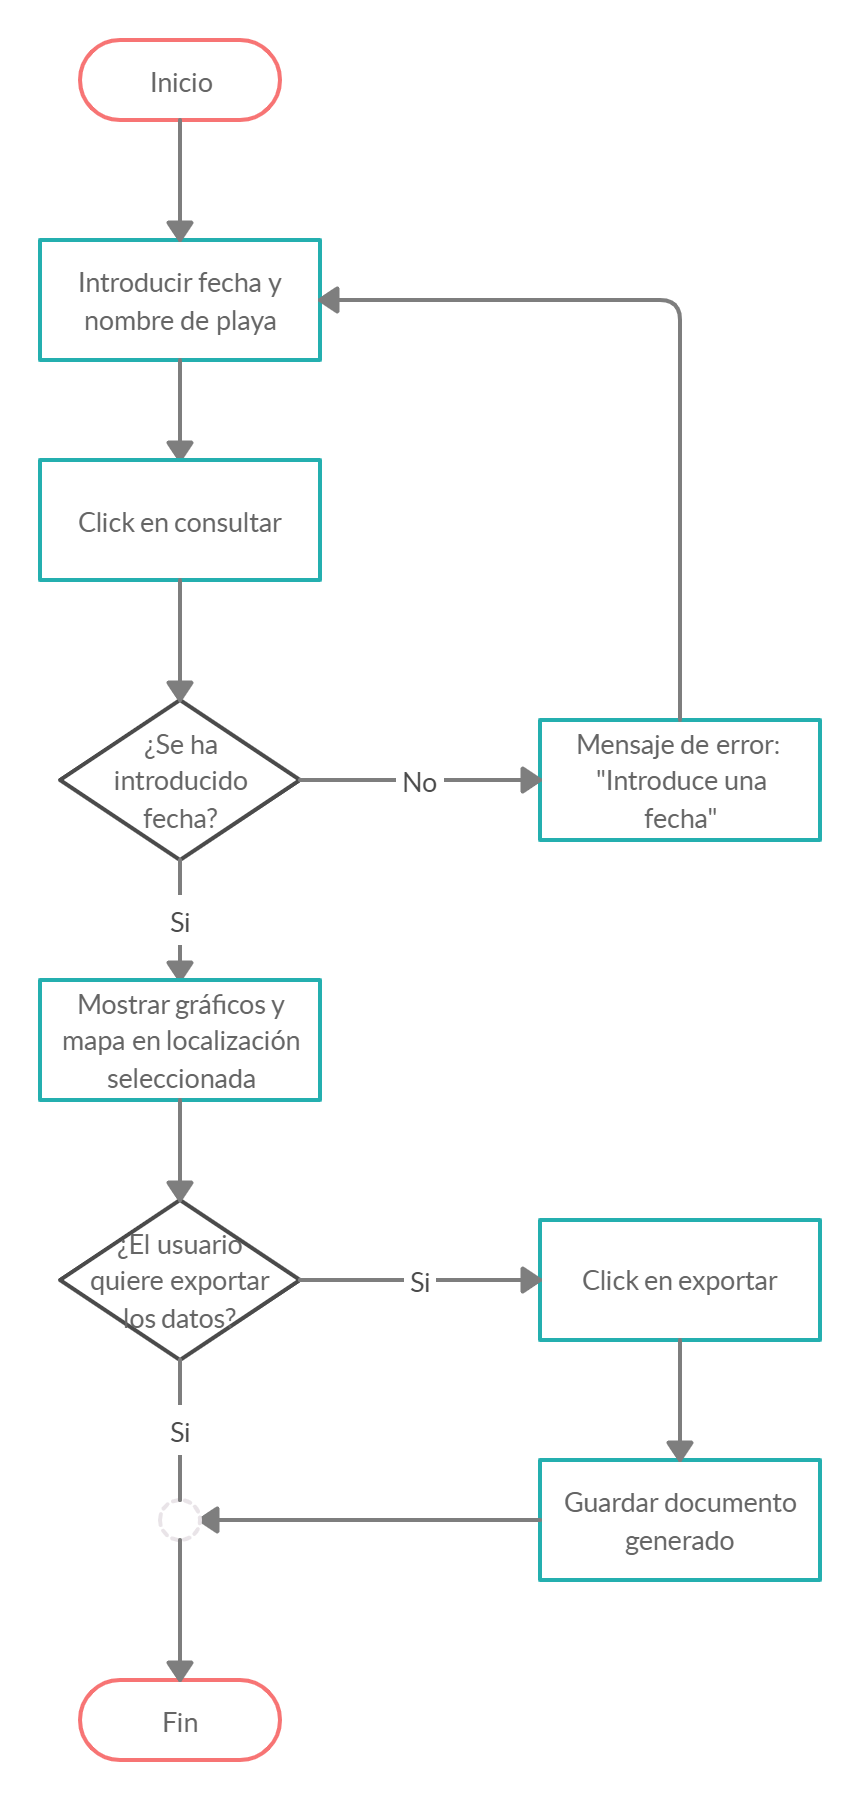
\includegraphics[width=0.6\textwidth]{diagramaFlujo.png}
	\caption{Diagrama de flujo}\label{fig:diagrama}
\end{figure}

\section{Diseño arquitectónico}

La arquitectura de la aplicación se puede considerar como un patrón Modelo-Vista-Controlador (MVC) \cite{mvc} en lo que nos encontramos tres elementos principales:

\begin{itemize}
	\item \textbf{Modelo:} Contiene un representación de los datos que utiliza el sistema y la lógica de negocio del mismo. Los datos suelen consultarse a una base de datos, en nuestro caso, los datos de consulta se encuentran en una serie de \emph{dataframes}.
	\item \textbf{Vista:} Se trata de la interfaz de usuario. Todo lo relacionado con la representación gráfica es responsabilidad de la vista.
	\item \textbf{Controlador:} Como su propio nombre indica es el encargado de controlar los eventos generados por el usuario. Es el encargado de solicitar los datos al modelo y enviárselos a la vista.
\end{itemize}

\begin{figure}[!h]
	\centering
	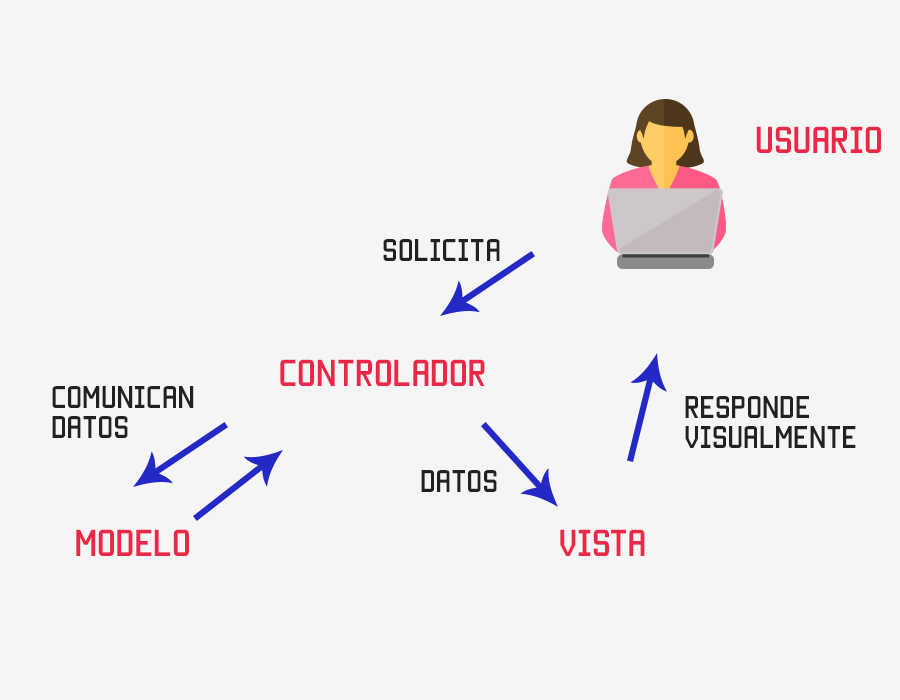
\includegraphics[width=0.6\textwidth]{mvc.jpg}
	\caption{Representación del patrón Modelo-Vista-Controlador}\label{fig:mvc}
\end{figure}



\section{Diseño de interfaces}

Anteriormente a la realización de la aplicación, se realizaron una serie de bocetos en los que se reflejaron las principales ideas. Para esto se utilizó la aplicación Pencil.

\begin{figure}[!h]
	\centering
	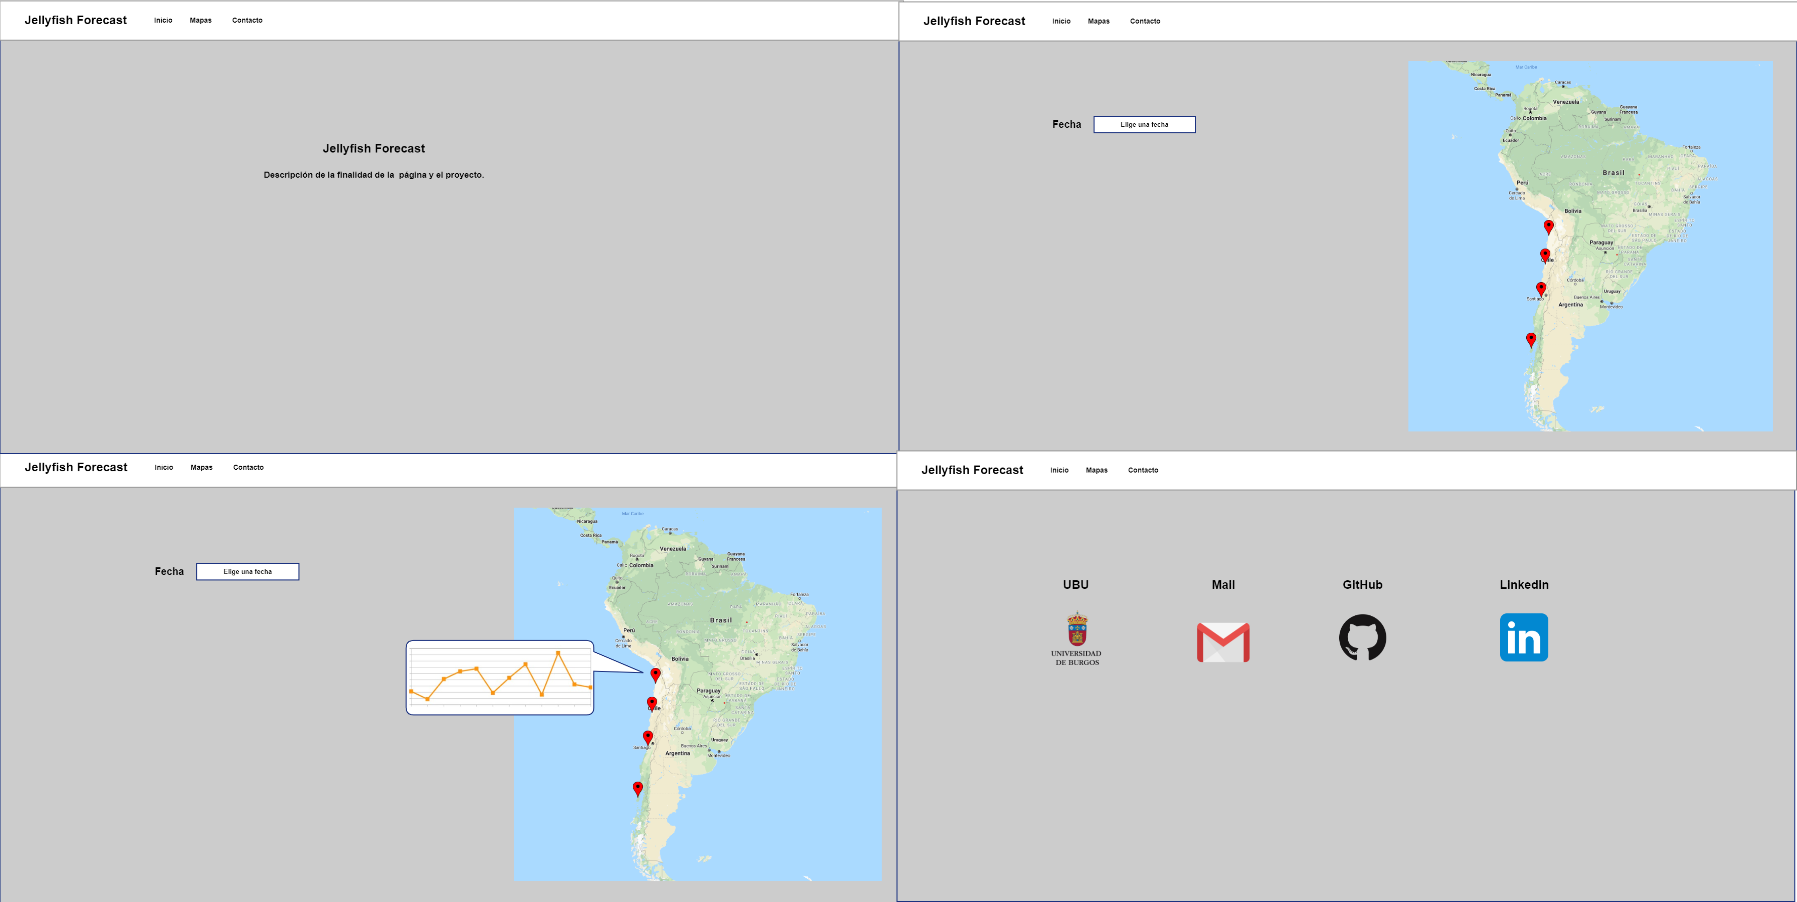
\includegraphics[width=1\textwidth]{bocetos.png}
	\caption{Bocetos iniciales}\label{fig:bocetos}
\end{figure}








\apendice{Documentación técnica de programación}

\section{Introducción}
En este apéndice se explicarán todos los aspectos relevantes del proyecto con el objetivo de facilitar la comprensión del mismo si otro desarrollador quisiera continuar con el trabajo o entenderlo más a fondo.

\section{Estructura de directorios}

El proyecto está alojado en dos repositorios diferentes. El motivo, es el de conseguir un despliegue automático a través de la plataforma \emph{heroku}. Por lo que nos encontramos con:

\subsection{Web Jellyfish Forecast}
Es el repositorio\footnote{Web Jellyfish Forecast. \url{https://github.com/psnti/WebJellyfishForecast}} en el que se alojan todos los ficheros necesarios para el funcionamiento de la aplicación web.

Contiene los siguientes directorios:
\begin{itemize}
	\item \textbf{Documentos}: Se guardan, el dataframe en el que estan la relación de playas con sus coordenadas así como un fichero excel con los avistamientos, necesario para realizar el historial de avistamientos.
	\item \textbf{static}: Aloja los ficheros css y javascript así como las imágenes necesarios para el buen funcionamiento de la aplicación.
	\item \textbf{templates}: Contiene los ficheros html.
\end{itemize}

Tambien contiene los siguientes archivos:
\begin{itemize}
	\item \textbf{Procfile}: Archivo necesario para el despliegue en \emph{Heroku} que contiene el comando que debe ejecutar la app en el arranque.
	\item \textbf{app.py}: Archivo python con la funcionalidad de la aplicación.
	\item \textbf{requirements.txt}: Listado de bibliotecas que se deben instalar en la máquina antes de ejecutar la aplicación.
\end{itemize}

\subsection{Jellyfish Forecast}
Es el repositorio\footnote{Jellyfish Forecast. \url{https://github.com/psnti/Jellyfish_Forecast}} en el que se alojan el resto de archivos del proyecto.

Contiene los siguientes directorios:
\begin{itemize}
	\item \textbf{Web}: Contiene el boceto de la aplicación realizado antes del desarrollo de la misma asi como una referencia al anterior repositorio.
	\item \textbf{docs/latex}: Aloja la documentación del proyecto.
	\item \textbf{src}: Contiene todo el código utilizado para la descarga y tratamiento de los datos así como el entrenamiento del modelo.
\end{itemize}

\section{Manual del programador}

Este apartado está destinado a la explicación de la instalación de todo lo necesario para poder ejecutar el proyecto o programadores que quieran trabajar en la mejora del mismo.

Para la ejecución del proyecto es indispensable la instalación de Python (el desarrollo se ha realizado con la versión 3.7.6). Posteriormente se instalarán los paquetes recogidos en el fichero requirements.txt como se indica en el apartado \ref{D4}.

En cuanto a la generación del modelo la mayoría del código está elaborado con \emph{jupyter notebook} por lo que es necesaria su instalación. La manera más sencilla es instalando \emph{Anaconda}\footnote{Anaconda. \url{https://www.anaconda.com/products/individual}}.

\section{Compilación, instalación y ejecución del proyecto}\label{D4}

En este apartado se indicará el proceso de obtener proyecto desde el repositorio hasta su despliegue en la plataforma de \emph{Heroku}.

\subsection{Descargar el proyecto}\label{Descarga}

\begin{enumerate}
	\item En primer lugar se ha de acceder al repositorio\footnote{Web Jellyfish Forecast. \url{https://github.com/psnti/WebJellyfishForecast}}.
	\item Descargar el contenido desde \textbf{Clone or Download}
	\imagen{clone_download.png}{Descargar repositorio}\label{clone}
	\item Descomprimir el fichero .zip en la ruta deseada.
	\item Antes de instalar las bibliotecas utilizadas en el proyecto crearemos un entorno virtual y accederemos a el:
	\begin{verbatim}
	python -m venv env
	env\Scripts\active.bat
	\end{verbatim}
	\item Para la instalación de la biblioteca necesarias, contamos con el archivo requirements.txt. Ejecutando el siguiente comando, se instalarán todas las dependencias del proyecto en  nuestro entorno virtual.
	\begin{verbatim}
	pip install -r requirements.txt
	\end{verbatim}
	
\end{enumerate}

\subsection{Ejecutar aplicación}

\begin{enumerate}
	\item Una vez instaladas todas las dependencias, podremos ejecutar la aplicación. Desde el entorno virtual ejecutamos:
	\begin{verbatim}
	Flask run
	\end{verbatim}
	\item Accederemos desde el navegador a la dirección \href{http://127.0.0.1:5000}{http://127.0.0.1:5000}
	
\end{enumerate}

\subsection{Modificación de los datos}

Si se quisiera modificar el listado de playas que aparecen en la aplicación se deberá editar o sustituir el fichero ``listado\_playas.pkl'' contenido en el directorio ``documentos'' donde se recogen el nombre la playa con sus respectivas coordenadas. En este mismo directorio se encuentra el documento excel con los avistamientos de las medusas (``Datos\_Physalia\_20171010.xls'') y del que se extraen los datos para generar el gráfico del historial de cada playa. 

Si se modifica el fichero con el listado de las playas, los nombres de las mismas deberán coincidir con los que aparecen en el archivo excel si se quiere que el gráfico del historial tenga contenido.

En cuanto al modelo predictivo, se encuentra en la carpeta ``static''.

\subsection{Despliegue de la aplicación}

El despliegue se realizó en la plataforma \emph{Heroku} pues es gratuita y los recursos que ofrece son suficientes para los requisitos de nuestro proyecto.

Hay dos ficheros importantes para el despliegue:
\begin{itemize}
	\item \textbf{requirements.txt}: como se ha mencionado anteriormente, recoge todas las dependencias del proyecto y es necesario para que se instalen en la maquina antes de ejecutarlo. Si se añaden bibliotecas se deberá reflejar en este archivo. Dentro del entorno virtual ejecutaremos:
	\begin{verbatim}
	pip freeze > requirements.txt
	\end{verbatim}
	De esta manera se actualizarán todas la bibliotecas instaladas en el entorno virtual.
	\item En segundo lugar, el archivo \textbf{Procfile}. Contiene el comando que debe ejecutar la app en el arranque y debe ir sin extensión.
\end{itemize}


Una vez tengamos estos archivos deberemos seguir los siguientes pasos:
\begin{enumerate}
	\item Acceder a la pagina de \emph{Heroku}\footnote{Heroku \url{https://www.heroku.com/}} y crear una cuenta.
	\item Entraremos en nuestra cuenta, y en el panel de usuario crearemos una nueva \emph{app}.
	\begin{figure}[!h]
		\centering
		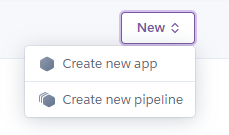
\includegraphics[width=0.6\textwidth]{new_app.png}
		\caption{Nueva app en \emph{Heroku}}\label{fig:new_app}
	\end{figure}
	\item Añadimos un nombre para nuestra aplicación y ya tendremos nuestra app creada.
	\begin{figure}[!h]
		\centering
		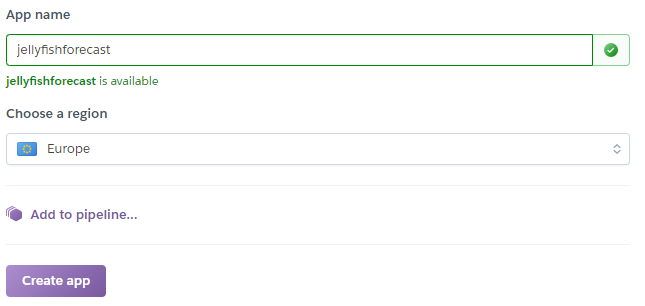
\includegraphics[width=0.9\textwidth]{nombre_app.png}
		\caption{Nombrar nueva app en \emph{Heroku}}\label{fig:new_app}
	\end{figure}
	\item A la hora de realizar el despliegue tendremos dos opciones: asociar la aplicación a un repositorio existente de \emph{GitHub}, o crear un nuevo repositorio en \emph{Heroku}. En el caso de este proyecto se eligió la opción de asociarlo a un repositorio en \emph{GitHub}. 
	
	Si se prefiriese el repositorio en \emph{Heroku} las instrucciones para su creación aparecen en la pagina de la aplicación.
	\begin{figure}[!h]
		\centering
		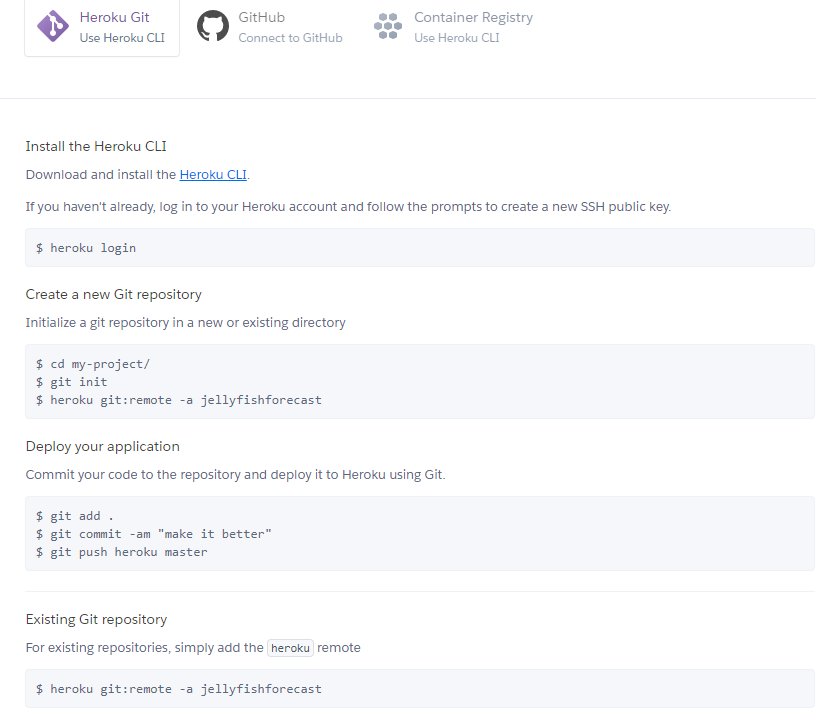
\includegraphics[width=0.9\textwidth]{deploy_heroku.png}
		\caption{Modos de despliegue en \emph{Heroku}}\label{fig:deploy}
	\end{figure}
		
\end{enumerate}

\subsection{Generación del modelo}

La generación del modelo y las pruebas están recogidas en el segundo repositorio\footnote{Jellyfish Forecast. \url{https://github.com/psnti/Jellyfish_Forecast}}. La forma de descargarlo e instalar todas las bibliotecas necesarias es igual a lo explicado en el anterior repositorio.

En la carpeta ``scr/Descarga datos'' podremos encontrar dos scripts diferentes para poder descargar los datos oceánicos de origen desde \emph{Copernicus}. Uno lo hace a través de una API. Esta opción se descartó, pues en el momento de descargar los datos era bastante nueva y originaba errores, además de tardar demasiado en generar los paquetes de datos. El otro, descarga los datos a través de un FTP. Esta opción descarga un volumen mucho mayor pues se descargan los datos de cada dia y de todo el mundo, por lo que tras descargar cada archivo, el script realiza un \emph{crop} dejando unicamente el área de Chile y las variables que nos interesan para el estudio como se explica en el apartado \ref{diseño_datos}

Si nos movemos a la carpeta ``src/Avistamientos'' nos encontramos con los \emph{notebooks} utilizados para la generación del modelo predictivo.
\begin{itemize}
	\item En la carpeta ``\textbf{\#ExcelsAvistamientosIniciales}'' encontraremos los conjuntos de datos de los avistamientos. La versión más reciente es ``Datos\_Physalia\_20171010.xls''.
	\item El archivo GenerarEstructura.ipynb realiza todo el trabajo de tratar los conjuntos de datos, unirles y generar una estructura que posteriormente se utilizará para entrenar al modelo. Estas estructuras se guardan en dos formatos distintos. En la carpeta ``Excels'' están los archivos con formato .xlsx para consulta, pues son más fáciles de visualizar. Por otro lado, en la carpeta ``pkls'' se encuentran los archivos con formato .pkl que son con los que se trabaja pues su lectura y guardado son más eficientes de leer y guardar.
	\item La carpeta ``PruebasGeneracionEstructuraDatos'' contiene varios \emph{notebooks} con pruebas de las diferentes transformaciones que se han realizado a la estructura de datos. 
	\item Por ultimo, ``GeneracionModelo'' contiene algunas pruebas que se realizaron a la hora del aprendizaje con \emph{Scikit-learn} y tres \emph{notebooks} con las  pruebas realizadas con diferentes algoritmos.
\end{itemize}

\section{Pruebas del sistema}

\subsection{Pruebas de funcionamiento}
A parte de las pruebas por parte de los usuarios, se han realizado pruebas automáticas utilizando la herramienta \emph{Selenium}.

Se ha utilizado la biblioteca para Python con el driver correspondiente para Google Chrome. Elegí esta opción en vez de utilizar la extensión disponible debido a tener una breve experiencia con esta biblioteca. 

La versión de Chrome con la que se ha utilizado ha sido la 83.0.4103.106 con el driver correspondiente para esta versión. Si se prueba en el futuro, es probable que la versión del navegador sea diferente. Habría que descargar la versión correspondiente del driver, e introducirla en la carpeta ``test/chromedriver'' del repositorio \emph{WebJellyfishForecast}.

Para ejecutar las pruebas, accederemos el entorno virtual como se ha explicado en el punto anterior y ejecutaremos el fichero \emph{test.py}.
\begin{verbatim}
Python test/test.py
\end{verbatim}

Esta ejecución genera un fichero ``test.log'' con las salida de los test.


\subsection{Pruebas del modelo}
\textcolor{red}{diferentes algoritmos}



\apendice{Documentación de usuario}

\section{Introducción}

%Este apéndice recoge todo lo que un usuario debe saber para poder ejecutar la aplicación. Cabe destacar que para un cualquier usuario no seria necesario la instalación de ninguna herramienta pues la aplicación está desplegada\footnote{Página web Jellyfish Forecast. \url{https://jellyfish-forecast.herokuapp.com/}} y puede visitarse desde cualquier navegador. A pesar de ello, se explicará como instalar y ejecutar la aplicación desde un servidor local.

Este apéndice recoge todo lo que un usuario debe saber para poder ejecutar la aplicación y los requisitos mínimos que se necesitan. 

\section{Requisitos de usuarios}
%Para la ejecución de la aplicación se deberá tener instalado Python (el desarrollo se ha realizado con la versión 3.7.6). Posteriormente se instalarán los paquetes recogidos en el fichero requirements.txt. La realización del proyecto ha sido en una máquina con sistema operativo W10, pero debería poder ejecutarse en otros sistemas sin problemas.
La aplicación se encuentra desplegada por lo que la única instalación necesaria seria la de un navegador web. En el apartado de pruebas de la aplicación se recogen algunos navegadores que han sido probados y funcionan correctamente \ref{pruebas_navegadores}.

%\section{Instalación}
%
%Para la instalación de el proyecto se deberán seguir los siguientes pasos. Estos pasos son los mismos que los recogidos en el apéndice anterior \ref{Descarga} con un menor detalle:
%
%\begin{enumerate}
%	\item En primer lugar se ha de acceder al repositorio\footnote{Web Jellyfish Forecast. \url{https://github.com/psnti/WebJellyfishForecast}}.
%	\item Descargar el contenido desde \textbf{Clone or Download}
%	\imagen{clone_download.png}{Descargar repositorio}\label{clone}.
%	\item Descomprimir el fichero .zip en la ruta deseada.
%	\item Antes de instalar las bibliotecas utilizadas en el proyecto crearemos un entorno virtual y accederemos a el:
%	\begin{verbatim}
%	python -m venv env
%	env\Scripts\active.bat
%	\end{verbatim}
%	\item Para la instalación de la biblioteca necesarias, contamos con el archivo requirements.txt. Ejecutando el siguiente comando, se instalarán todas las dependencias del proyecto en  nuestro entorno virtual.
%	\begin{verbatim}
%	pip install -r requirements.txt
%	\end{verbatim}
%\end{enumerate}

\section{Manual del usuario}

Una vez dentro de la web ya sea ejecutándolo en un servidor local, o desde
la página desplegada,las acciones se realizan de la misma manera.

En primer lugar nos encontramos con una página de inicio meramente informativa.

\imagen{pagina_inicio_web.png}{Página de inicio}\label{pagina_inicio}

Desde ahí, podremos acceder a la pestaña de <<Mapas>> donde se encuentra la funcionalidad de la aplicación.

\imagen{pagina_mapas_web.png}{Página de consulta}\label{pagina_mapas_web}

Para realizar una predicción, deberemos introducir una fecha y una playa. En caso de seleccionar unicamente una playa sin fecha, aparecerá un mensaje de error indicándonoslo.

\imagen{pagina_error_fecha.png}{Error en la consulta}\label{pagina_error_fecha}

Una vez seleccionadas ambas opciones correctamente, al hacer click en <<Consultar>> nos aparecerán dos gráficos y el mapa realizará un zoom a la playa seleccionada. Estos gráficos se tratan, de la predicción realizada y el historial de avistamientos de la playa seleccionada. 

\imagen{pagina_consulta.png}{Página de consulta con gráficos}\label{pagina_consulta}

Una vez realizada la predicción, existe la opción de exportar dicha predicción a un fichero de tipo .xlsx

\textcolor{red}{imagen fichero exportado}

Por último, nos encontramos la pestaña de contacto donde se sitúan enlaces a la página de la Universidad, el repositorio y enlaces de contacto.

\imagen{pagina_contacto.png}{Página de contacto}\label{pagina_contacto}


\bibliographystyle{plain}
\bibliography{bibliografiaAnexos}

\end{document}
